\documentclass[12pt,a4paper,oneside]{report}

\usepackage[T1]{fontenc}
\usepackage[utf8]{inputenc}
\usepackage[ngerman]{babel}
\usepackage[a4paper,margin=2.6cm]{geometry}
\usepackage{graphicx}
\usepackage{longtable}
\usepackage{array}
\usepackage{listings}
\usepackage{amssymb}
\usepackage{csquotes}
\usepackage{xcolor}
\usepackage{hyperref}
\usepackage{enumitem}
\usepackage{lmodern}
\usepackage{microtype}
\usepackage{fancyhdr}
\usepackage{setspace}
\usepackage{titlesec}

\definecolor{dmTECHcolor}{RGB}{75,55,140}
\definecolor{codebg}{rgb}{0.95,0.95,0.92}
\definecolor{codeframe}{RGB}{190,190,190}
\definecolor{codekeyword}{rgb}{0.58,0,0.82}
\definecolor{codetype}{RGB}{31,54,133}
\definecolor{codecomment}{rgb}{0.5,0.5,0.5}
\definecolor{codestring}{rgb}{0,0.6,0}
\definecolor{codenumber}{rgb}{0.5,0.5,0.5}

\newcommand{\Titel}{Programmentwurf - Protokoll}
\newcommand{\Untertitel}{PICasso -- PIC Microcontroller Simulator}
\newcommand{\Autor}{Nik Wachsmann und Ben Stahl}
\newcommand{\AbgabeDatum}{04.05.2026}

\hypersetup{
    colorlinks=true,
    linkcolor=dmTECHcolor,
    urlcolor=dmTECHcolor,
    citecolor=dmTECHcolor,
    filecolor=dmTECHcolor,
    bookmarks=true,
    bookmarksopen=true,
    bookmarksnumbered=true,
    unicode=true,
    pdfstartview={FitV}
}

\pagestyle{fancy}
\fancyhf{}
\fancyhead[L]{\nouppercase{\leftmark}}
\fancyhead[R]{\Autor}
\fancyfoot[C]{\thepage}
\setlength{\headheight}{15pt}
\fancypagestyle{plain}{
    \fancyhf{}
    \fancyhead[L]{\nouppercase{\leftmark}}
    \fancyhead[R]{\Autor}
    \fancyfoot[C]{\thepage}
}

\lstdefinelanguage{bash}{
    sensitive=true,
    morekeywords={cd,cmake,make,git,mkdir},
    alsoletter={-},
    morecomment=[l]{\#},
    morestring=[b]",
    morestring=[b]'
}

\lstdefinelanguage{picassocpp}[]{C++}{
    morekeywords=[2]{
        uint8_t,uint16_t,uint32_t,uint64_t,
        int8_t,int16_t,int32_t,int64_t,
        size_t,bool,string,
        Bit,Nibble,Byte,Register,Ram,Stack,MemoryInterface,
        IMemoryInterface,Instruction,Arithmetic,Bitwise,Jump,Literal,
        ALU,Compiler,Program,Timer,Prescaler,PIC,PICDebugInterface,
        TerminalUI,Logger,FakeMemoryInterface,FakeProgram,
        ADDWF,SUBWF,DECF,INCF,BCF,BSF,BTFSC,BTFSS,GOTO,CALL,
        MOVLW,ADDLW,CLRWDT,RETFIE,RETURN,SLEEP
    }
}

\lstdefinestyle{codeblock}{
    basicstyle=\ttfamily\footnotesize,
    breaklines=true,
    frame=single,
    framerule=0.6pt,
    rulecolor=\color{codeframe},
    backgroundcolor=\color{codebg},
    columns=fullflexible,
    keepspaces=true,
    showstringspaces=false,
    numbers=left,
    numberstyle=\tiny\color{codenumber},
    numbersep=5pt,
    xleftmargin=1.0em,
    framexleftmargin=1em,
    keywordstyle=\color{codekeyword},
    keywordstyle=[2]\color{codetype}\bfseries,
    commentstyle=\color{codecomment},
    stringstyle=\color{codestring},
    identifierstyle=\color{black},
    literate=
        {ä}{{\"a}}1
        {ö}{{\"o}}1
        {ü}{{\"u}}1
        {Ä}{{\"A}}1
        {Ö}{{\"O}}1
        {Ü}{{\"U}}1
        {ß}{{\ss}}1
        {–}{{--}}1
        {≥}{{$\geq$}}1
        {→}{{$\rightarrow$}}1
}

\newcommand{\code}[1]{\texttt{\detokenize{#1}}}
\newcommand{\umlplaceholder}[1]{
    \begin{center}
        \fbox{\parbox{0.9\textwidth}{\centering\textit{#1}}}
    \end{center}
}

\setlist[itemize]{topsep=4pt,itemsep=2pt}
\setlist[enumerate]{topsep=4pt,itemsep=2pt}
\onehalfspacing
\setlength{\parindent}{0pt}
\setlength{\parskip}{0.35em}
\setcounter{tocdepth}{2}
\setcounter{secnumdepth}{3}

\renewcommand{\chaptername}{Kapitel}
\titleformat{\chapter}[display]
    {\bfseries\Huge\color{dmTECHcolor}}
    {\filleft\fontsize{42}{42}\selectfont\thechapter}
    {0.4ex}
    {\titlerule\vspace{1ex}\filright}
    [\vspace{1ex}\titlerule]
\titlespacing*{\chapter}{0pt}{0pt}{20pt}

\begin{document}

\begin{titlepage}
    \begin{center}
        \vspace*{-1.5cm}
        {\Huge \Titel\par}
        \vspace{0.8cm}
        \begin{doublespace}
            {\Huge \Untertitel\par}
        \end{doublespace}
        \vspace{0.8cm}
        {\large von\par}
        \vspace{0.4cm}
        {\large\bfseries \Autor\par}
        \vspace{0.8cm}
        {\large Abgabedatum \AbgabeDatum\par}
        \vfill
    \end{center}
    \begin{tabular}{l@{\hspace{2cm}}l}
        Matrikelnummer Nik Wachsmann & 1152312 \\
        Matrikelnummer Ben Stahl & 8238700 \\
    \end{tabular}
\end{titlepage}

\pagenumbering{roman}
\tableofcontents
\clearpage
\pagenumbering{arabic}

\chapter{Einführung}

\section{Übersicht über die Applikation}

\textbf{PICasso} ist ein Simulator für PIC-Midrange-Mikrocontroller, geschrieben in C++17.
Die Applikation liest assemblierte PIC-Programme im \code{.LST}-Format ein und führt diese Instruktion für Instruktion aus.
Dabei werden alle wesentlichen Hardwarekomponenten des PIC simuliert:
ein 2-Bank-RAM mit Registerspiegelung, ein 8-Bit-W-Akkumulator, ein 8-Level-Hardware-Stack, ein Timer/Prescaler-Subsystem
sowie die vollständige Ausführung aller 35 PIC-Midrange-Instruktionen.
Die Applikation bietet eine interaktive Terminal-Oberfläche (ncurses), über die der Benutzer Programme laden,
schrittweise oder im Dauerlauf ausführen, RAM-Inhalte inspizieren und modifizieren sowie einzelne Bits umschalten kann
Die Simulation läuft in einem separaten Thread, während die UI im Hauptthread rendert -- synchronisiert über atomare Flags und Mutexe.

\textbf{Zweck:} PICasso löst das Problem, PIC-Assemblerprogramme ohne physische Hardware testen und debuggen zu können.
Es dient als Lern- und Entwicklungswerkzeug für eingebettete Systeme.

\section{Starten der Applikation}

\textbf{Voraussetzungen:}

\begin{itemize}
    \item C++17-kompatibler Compiler (z.B. g++ $\geq$ 9)
    \item CMake $\geq$ 3.14
    \item ncurses-Bibliothek (\code{libncurses-dev} unter Linux)
\end{itemize}

\textbf{Schritt-für-Schritt-Anleitung:}

\begin{lstlisting}[style=codeblock,language=bash]
# 1. Repository klonen / Projektverzeichnis wechseln
git clone https://github.com/DefinitlyNotABot/PICasso.git
cd PICasso

# 2. Build-Verzeichnis erstellen und CMake konfigurieren
mkdir -p build && cd build
cmake ..

# 3. Projekt kompilieren
make

# 4. Simulator starten
./PICasso

# 5. Tests ausführen (optional)
cd ..
./build/AllTests
\end{lstlisting}

Nach dem Start öffnet sich die ncurses-Oberfläche.
Über den \emph{Load}-Button kann eine \code{.LST}-Datei aus dem \code{progs/}-Verzeichnis geladen werden.
Anschließend kann das Programm mit \emph{Step}, \emph{Run} (Dauerlauf) oder \emph{Dash} (Schnelllauf) ausgeführt werden.

\section{Technischer Überblick}

\begin{longtable}{|p{0.18\textwidth}|p{0.22\textwidth}|p{0.5\textwidth}|}
\hline
\textbf{Technologie} & \textbf{Beschreibung} & \textbf{Begründung} \\
\hline
C++17 & Primäre Programmiersprache & Bietet hardwarenahe Kontrolle, geeignet für Simulator-Entwicklung;
unterstützt \code{std::optional}, \code{std::shared_ptr}, \code{std::filesystem} und strukturierte Bindings. \\
\hline
CMake & Build-System & Plattformunabhängiges Build-System;
ermöglicht automatisches Herunterladen von Abhängigkeiten (Catch2) via \code{FetchContent}. \\
\hline
ncurses & Terminal-UI-Bibliothek & Ermöglicht eine interaktive TUI ohne grafische Abhängigkeiten;
ideal für ein konsolenbasiertes Debugging-Tool. Unterstützt Farben, Mauseingabe und Fenstermanagement. \\
\hline
Catch2 & Unit-Test-Framework & Header-only-Framework mit BDD-Stil (\code{TEST_CASE}/\code{SECTION});
automatische Testregistrierung und Generatoren (\code{GENERATE}). \\
\hline
nlohmann/json & JSON-Parsing für Testdateien & Erlaubt deklarative Testspezifikation in JSON-Dateien;
einfache Integration als Header-only-Bibliothek. \\
\hline
\code{std::thread / std::mutex / std::atomic} & Multithreading & Simulation und UI laufen parallel;
atomare Flags steuern den Simulationszustand. \\
\hline
\end{longtable}


\chapter{Softwarearchitektur}

\section{Clean Architecture}

Die Applikation orientiert sich an einer geschichteten Architektur, die Elemente der Clean Architecture aufgreift:

\begin{itemize}
    \item \textbf{Domain / Entities (innerster Ring):}
    Die Memory-Abstraktion (\code{Bit}, \code{Nibble}, \code{Byte}, \code{Register}) sowie \code{Ram}, \code{Stack} und \code{MemoryInterface}.
    Diese Klassen modellieren die Hardwaredomäne des PIC-Mikrocontrollers und haben keine Abhängigkeiten zu Framework- oder UI-Code.
    \item \textbf{Use Cases / Application Layer:} \code{Instruction} (mit allen 35+ Unterklassen), \code{ALU}, \code{Compiler},
    \code{Program}, \code{Timer}, \code{Prescaler} und \code{PIC}. Diese Schicht orchestriert die Simulation und nutzt die Domain-Klassen.
    \item \textbf{Interface Adapters:} \code{Filereader} (Dateisystem-Zugriff), \code{Logger} (Ausgabe-Abstraktion).
    \item \textbf{Frameworks / UI (äußerster Ring):} \code{TerminalUI}, \code{TUI_Renderer},
    \code{TUI_Controller} und alle TUI-Hilfsklassen. Diese hängen von ncurses ab und nutzen \code{PICSnapshot} als Daten-Transfer-Objekt.
\end{itemize}

\begin{center}
    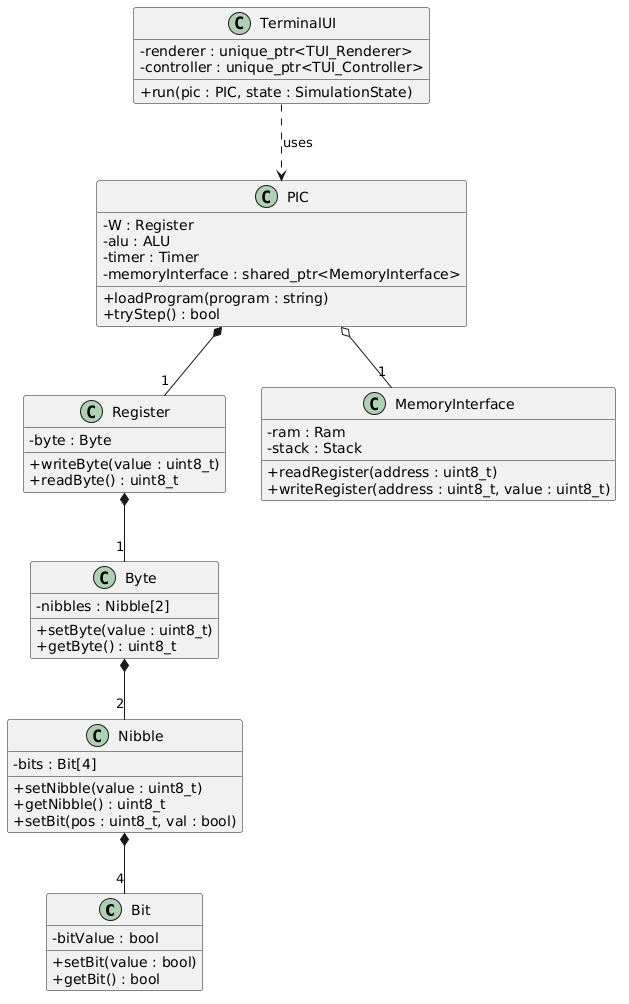
\includegraphics[width=0.9\textwidth]{UML/1.png}
\end{center}

\section{Domain Code}

\textbf{Domain Code} ist Code, der die überall gültige Logik der Anwendungsdomäne abbildet, unabhängig von Frameworks, Datenbanken oder UI.
Er ist der innere Teil der Anwedung, der sich selten ändern sollte. Im Fall von PICasso ist die Domäne die PIC-Mikrocontroller-Hardware.

\textbf{Beispiel:} Die Klasse \code{Stack} (\code{header/stack.hpp}) modelliert den 8-Level-Hardware-Stack des PIC. Sie hat keine Abhängigkeiten zu externen Bibliotheken und bildet rein fachliche Hardware-Logik ab:

\begin{lstlisting}[style=codeblock,language=picassocpp]
class Stack {
    private:
        uint8_t stack[8];
        uint8_t stackPointer;
    public:
        Stack();
        void push(uint8_t value);
        uint8_t pop();
        void reset();
};
\end{lstlisting}

\section{Analyse der Dependency Rule}
\subsection{Positiv-Beispiel: Dependency Rule}

Die Klasse \code{Register} (Domain/Entity) hat keine Abhängigkeiten zu äußeren Schichten.
Sie hängt nur von \code{Byte} ab, welches wiederum nur von \code{Nibble} und \code{Bit} abhängt welche alle innerhalb der Domain-Schicht sind.
Die äußere Schicht \code{Ram} hängt von \code{Register} ab, aber \code{Register} weiß nichts von \code{Ram}.
Die Abhängigkeit zeigt korrekt von außen nach innen.

\begin{center}
    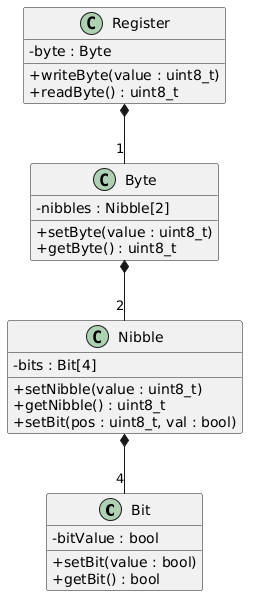
\includegraphics[width=0.5\textwidth]{UML/2.png}
\end{center}

\subsection{Negativ-Beispiel: Dependency Rule}

Die abstrakte Klasse \code{Instruction} (Application Layer) hat ein \textbf{statisches} Feld \code{static std::shared_ptr<MemoryInterface> memoryInterface},
das durch die \code{PIC}-Klasse gesetzt wird.
Das bedeutet, dass die Application-Layer-Klasse \code{Instruction} direkt an die konkrete Implementierung \code{MemoryInterface} gekoppelt ist.
Zudem wird das statische Feld von \code{PIC} (einem Orchestrator) gesetzt was zu einer impliziten Abhängigkeit von außen nach innen, 
die zur Laufzeit besteht, obwohl die Instruction-Klasse eigentlich keine Kenntnis über PIC haben sollte, führt.

\textbf{Lösung:} Dependency Injection -- die \code{MemoryInterface}-Referenz sollte als Konstruktor-Parameter an jede Instruction übergeben werden, statt über ein statisches Feld.

\begin{center}
    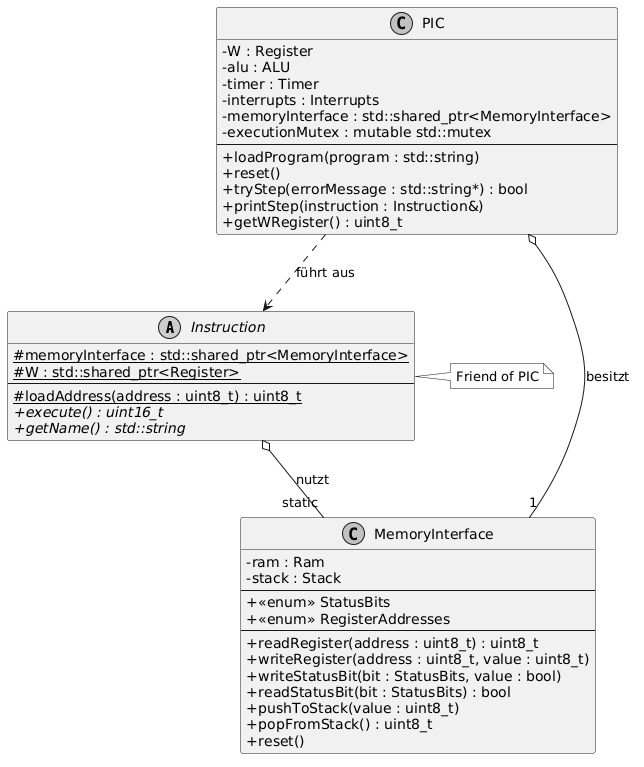
\includegraphics[width=0.9\textwidth]{UML/3.png}
\end{center}


\chapter{SOLID}

\section{Analyse SRP}

\subsection{Positiv-Beispiel}

\textbf{Klasse: \code{Stack}} (\code{header/stack.hpp})

Die Klasse \code{Stack} hat genau eine Verantwortlichkeit: die Verwaltung eines 8-Level-LIFO-Stacks für Rücksprungadressen. Sie bietet ausschließlich \code{push()}, \code{pop()} und \code{reset()}. Es gibt keinen Grund, diese Klasse zu ändern, außer wenn sich die Stack-Logik des PIC ändert -- also genau ein Änderungsgrund.

\begin{center}
    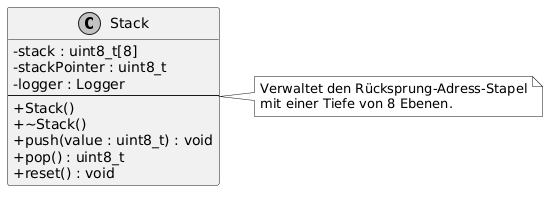
\includegraphics[width=0.9\textwidth]{UML/4.png}
\end{center}

\subsection{Negativ-Beispiel}

\textbf{Klasse: \code{PIC}} (\code{header/pic.hpp})

Die \code{PIC}-Klasse ist ein \enquote{God Object} mit mehreren Verantwortlichkeiten:

\begin{enumerate}
    \item Simulationsorchestrierung (Instruktionsausführung, Timer-Schritte)
    \item Programmmanagement (Laden, Kompilieren)
    \item Thread-sichere Zustandsabfragen für die UI (\code{getSnapshot()})
    \item Zustandsmanipulation für Debugging (\code{tryWriteRegister()}, \code{tryToggleBit()})
    \item Initialisierung aller Komponenten (Prescaler, Timer, statische Felder von \code{Instruction})
\end{enumerate}

\begin{lstlisting}[style=codeblock,language=picassocpp]
class PIC {
    ALU alu;
    Program loadedProgram;
    Register W;
    Timer timer;
    std::shared_ptr<MemoryInterface> memoryInterface;
    std::shared_ptr<Prescaler> prescaler;
    uint64_t totalSimulatedTimeUs;
    mutable std::mutex executionMutex;
    Logger logger;
    // ... 15+ öffentliche Methoden
};
\end{lstlisting}

\textbf{Lösungsweg:} Die Klasse sollte aufgeteilt werden in:

\begin{itemize}
    \item \code{PICHardware} -- hält Register, RAM, Timer (Hardware-Zustand)
    \item \code{PICSimulator} -- orchestriert Instruktionsausführung
    \item \code{PICDebugInterface} -- bietet thread-sichere Zugriffsmethoden für die UI
\end{itemize}

\begin{center}
    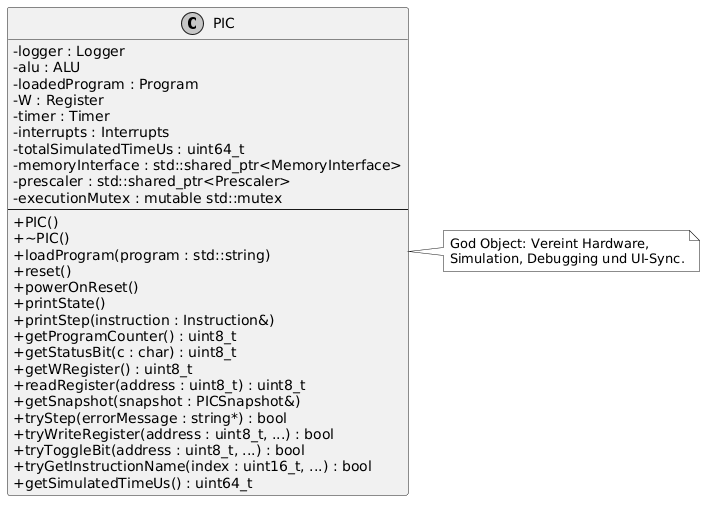
\includegraphics[width=0.9\textwidth]{UML/51.png}
\end{center}

\begin{center}
    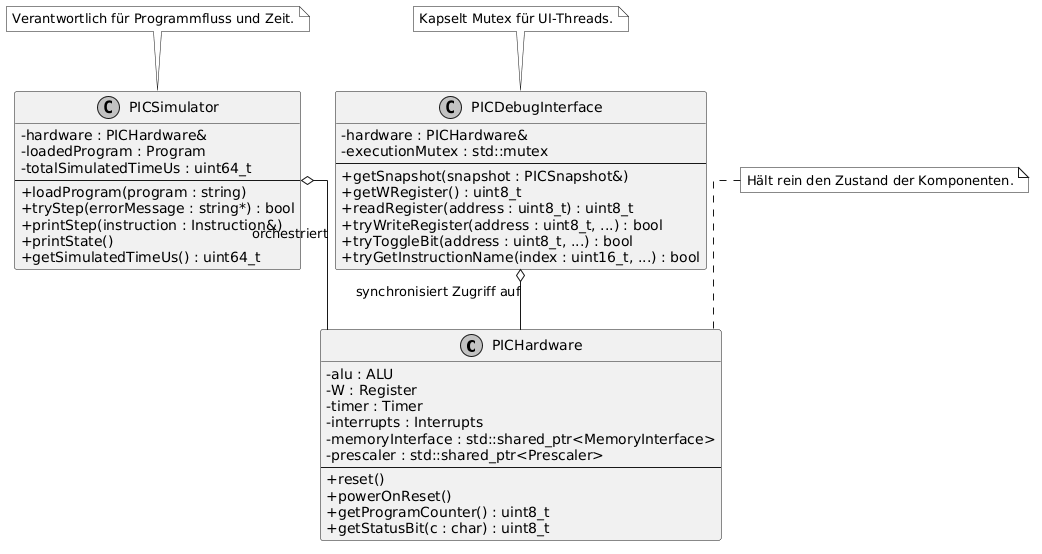
\includegraphics[width=0.9\textwidth]{UML/52.png}
\end{center}

\section{Analyse OCP}

\subsection{Positiv-Beispiel}

\textbf{Klasse: \code{Instruction}} (abstrakte Basisklasse, \code{header/instruction.hpp})

Die Klasse \code{Instruction} definiert die abstrakte Schnittstelle \code{virtual uint16_t execute() = 0}. Neue Instruktionstypen können durch Erstellen neuer Unterklassen hinzugefügt werden, ohne die Basisklasse zu modifizieren. Das Verhalten wird durch Vererbung erweitert. Beispiel: Um eine neue Instruktion hinzuzufügen, wird eine neue Klasse erstellt, die \code{Instruction} erbt und \code{execute()} implementiert.

\begin{lstlisting}[style=codeblock,language=picassocpp]
class Instruction {
    public:
        virtual uint16_t execute() = 0;   // offen für Erweiterung
        virtual std::string getName() = 0;
        virtual ~Instruction() = default;
};

class ADDWF : public Arithmetic {  // Erweiterung ohne Änderung der Basis
    public:
        uint16_t execute() override;
        std::string getName() override;
};
\end{lstlisting}

\begin{center}
    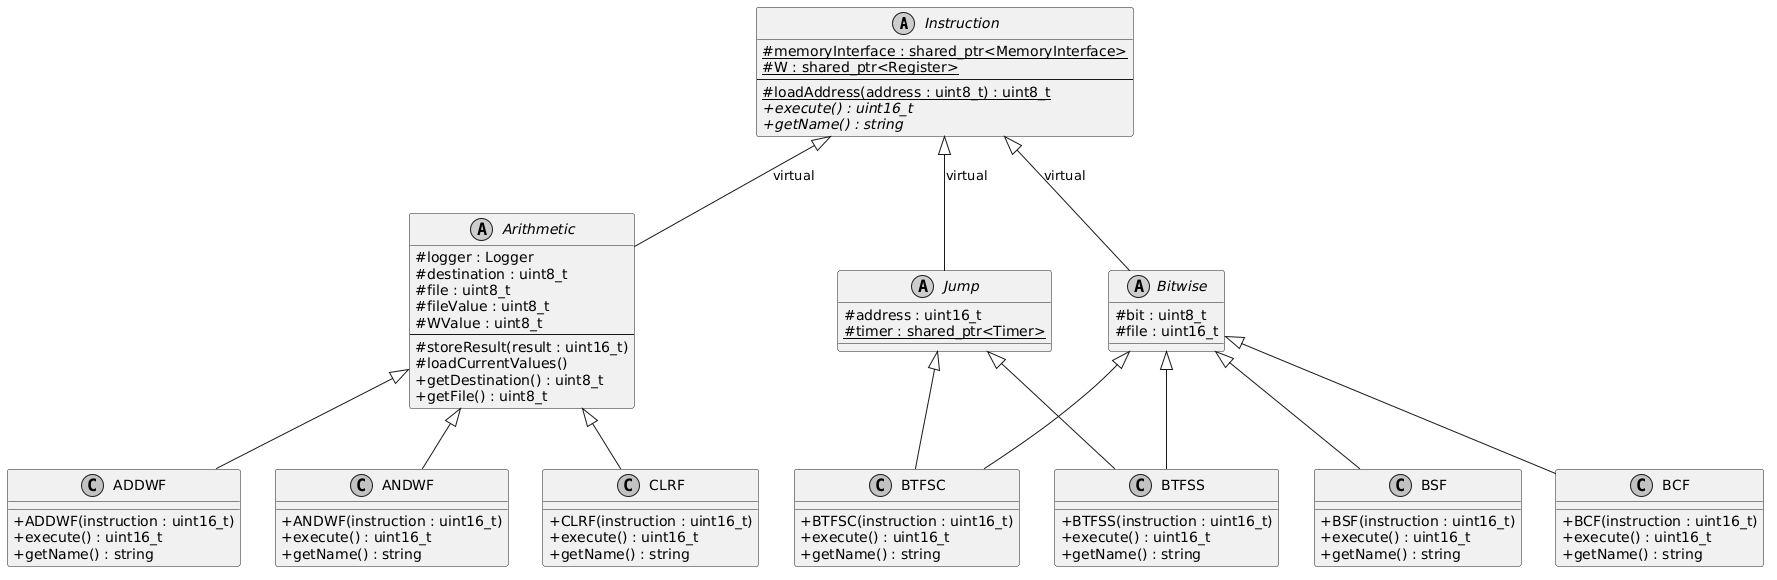
\includegraphics[height=0.5\textwidth, angle=90]{UML/6.png}
\end{center}

\subsection{Negativ-Beispiel}

\textbf{Klasse: \code{Compiler}} (\code{src/compiler.cpp})

Die Methode \code{Compiler::getInstruction()} enthält eine große Switch-Kaskade, die für jede Instruktion einen expliziten Case hat. Wenn eine neue Instruktion hinzugefügt wird, muss die Methode \code{getInstruction()} modifiziert werden -- ein klarer Verstoß gegen das Open/Closed Principle.

\begin{lstlisting}[style=codeblock,language=picassocpp]
std::unique_ptr<Instruction> Compiler::getInstruction(const uint16_t instruction) {
    switch(instruction) {
        case 0x0064: return std::make_unique<CLRWDT>(instruction);
        case 0x0009: return std::make_unique<RETFIE>(instruction);
        case 0x0008: return std::make_unique<RETURN>(instruction);
        case 0x0063: return std::make_unique<SLEEP>(instruction);
        // ... ~35 weitere Cases
    }
    // ... weitere Switch-Blöcke mit Bitmasks
}
\end{lstlisting}

\textbf{Lösung:} Ein Registry-Pattern / Factory-Map, bei der jede Instruktionsklasse sich selbst registriert:

\begin{lstlisting}[style=codeblock,language=picassocpp]
// Instruction-Factory mit Registry
using InstructionFactory = std::function<std::unique_ptr<Instruction>(uint16_t)>;
std::map<uint16_t, InstructionFactory> instructionRegistry;

// Registrierung in der jeweiligen Instruktionsklasse:
static bool registered = []() {
    instructionRegistry[0x0700] = [](uint16_t op) {
        return std::make_unique<ADDWF>(op);
    };
    return true;
}();
\end{lstlisting}


\begin{center}
    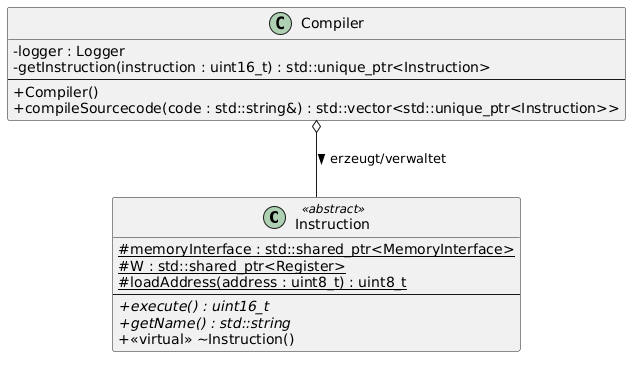
\includegraphics[width=0.9\textwidth]{UML/7.png}
\end{center}


\section{Analyse DIP}

\subsection{Positiv-Beispiel}

\textbf{Klasse: \code{ALU}} (\code{header/alu.hpp})

Die \code{ALU} hängt von der abstrakten Schnittstelle \code{Instruction} ab, nicht von konkreten Instruktionsimplementierungen. Die Methode \code{executeInstruction(Instruction&)} akzeptiert eine Referenz auf die abstrakte Basisklasse. Dadurch kann die ALU jede beliebige Instruktion ausführen, ohne konkrete Klassen zu kennen:

\begin{lstlisting}[style=codeblock,language=picassocpp]
class ALU {
    public:
        uint16_t executeInstruction(Instruction& instruction) {
            return instruction.execute();
        }
};
\end{lstlisting}

Die ALU hängt von der Abstraktion (\code{Instruction}) ab, nicht von den Details (\code{ADDWF}, \code{SUBWF}, etc.), was DIP konform ist.

\begin{center}
    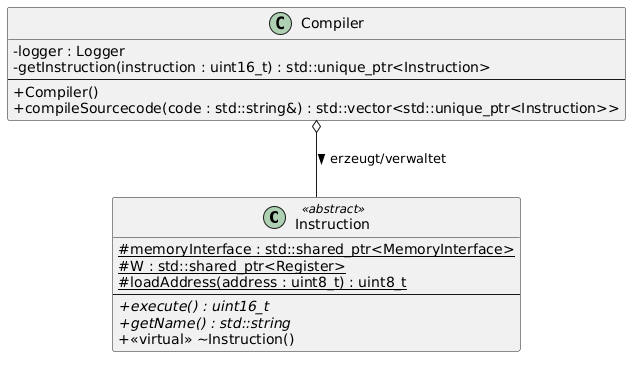
\includegraphics[width=0.9\textwidth]{UML/7.png}
\end{center}

\subsection{Negativ-Beispiel}

\textbf{Klasse: \code{PIC}}

Der PIC hängt direkt von der konkreten Implementierung des Registers ab.
Es gibt keine Abstraktionebene, gegen die Programmiert wird.
Für tests muss die konkrete Register Klasse verwendet wirden.

\begin{center}
    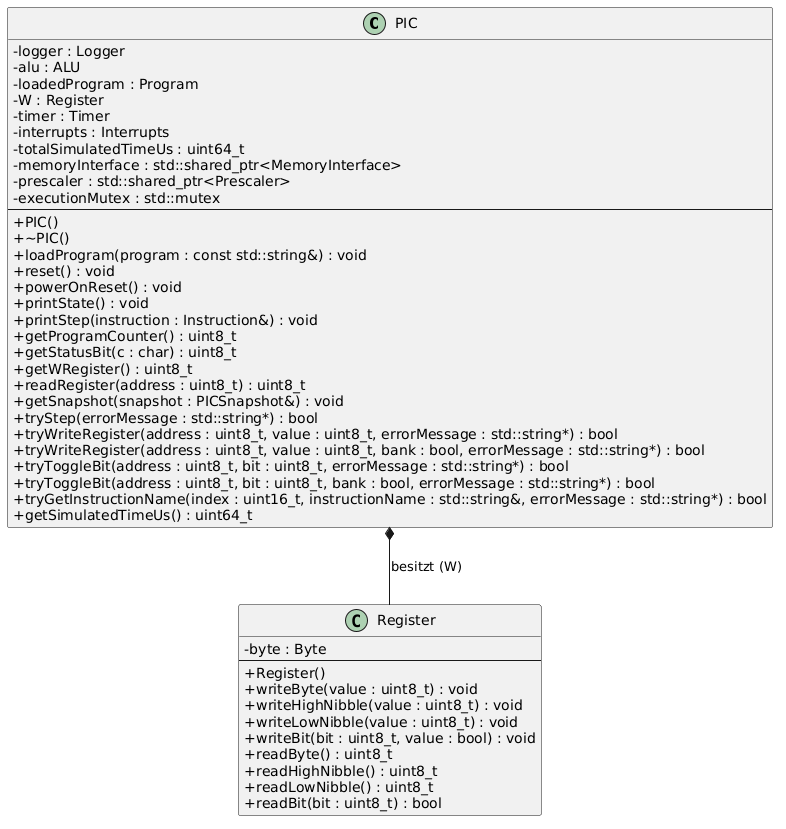
\includegraphics[width=0.9\textwidth]{UML/9.png}
\end{center}

Um dies Aufzulösen, kann eine abstrakte IRegister Klasse implementiert werden.

\begin{center}
    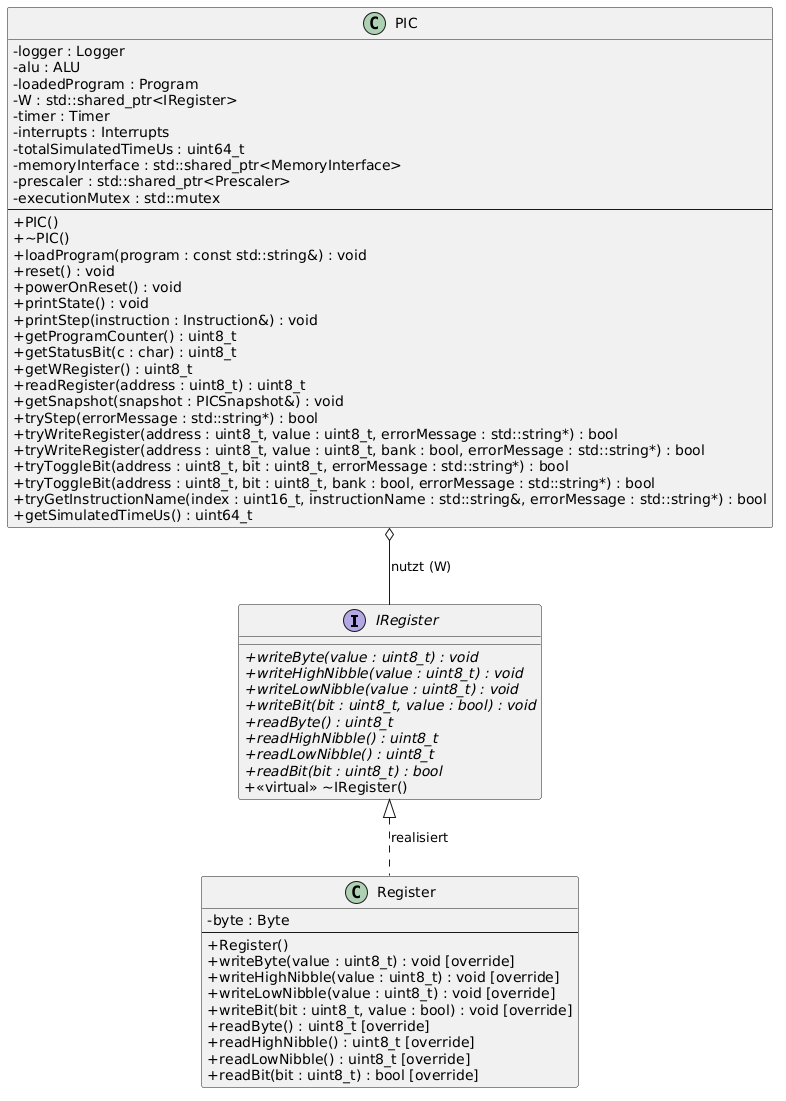
\includegraphics[width=0.9\textwidth]{UML/91.png}
\end{center}


\chapter{Weitere Prinzipien}

\section{Analyse GRASP: Geringe Kopplung}

\textbf{Klasse: \code{Filereader}} (\code{header/filereader.hpp})

Die Klasse \code{Filereader} hat eine minimale Kopplung zu anderen Klassen. Sie bietet eine einzige öffentliche Methode \code{readFile(filename) -> tuple<bool, string>}, die eine Datei liest und den Inhalt zurückgibt. Sie hat keine Abhängigkeiten zu PIC-spezifischen Klassen.

\textbf{Aufrufer:} Nur die Klasse \code{Program} nutzt \code{Filereader} in der Methode \code{loadProgram()}. Ebenso nutzt \code{TUI_Controller} sie indirekt über \code{Program}. Da \code{Filereader} nur Standard-C++-Bibliotheken verwendet und keine PIC-spezifischen Typen kennt, kann sie problemlos wiederverwendet oder ausgetauscht werden. Die Kopplung ist gering, weil:

\begin{itemize}
    \item Nur 1 Nutzer (\code{Program}) ist direkt abhängig
    \item Keine Kenntnis über die Domäne (PIC-Simulation)
    \item Rückgabewert ist ein generischer Typ (\code{tuple<bool, string>})
    \item Keine Abhängigkeiten zu anderen Projektklassen
\end{itemize}

\begin{center}
    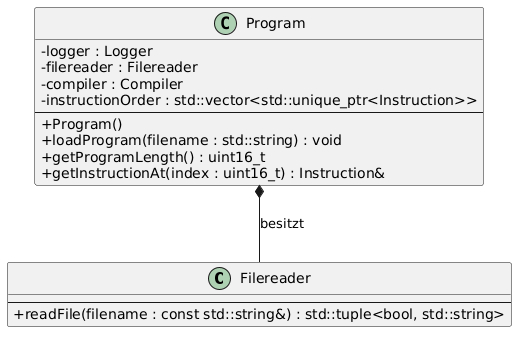
\includegraphics[width=0.9\textwidth]{UML/10.png}
\end{center}


\section{Analyse GRASP: Pure Fabrication}

\textbf{Klasse: \code{Logger}} (\code{header/logger.hpp})

Die Klasse \code{Logger} ist ein \textbf{Pure Fabrication} -- sie repräsentiert kein Konzept aus der PIC-Hardware-Domäne, sondern wurde ausschließlich aus softwaretechnischen Gründen erstellt, um eine einheitliche Logging-Infrastruktur bereitzustellen.

\textbf{Begründung des Einsatzes:} Ohne den Logger müsste jede Klasse ihre eigene Ausgabe-Logik implementieren (z.B. \code{std::cout}-Aufrufe), was zu Codeduplizierung führen würde. Der Logger bündelt die Verantwortlichkeit der Protokollierung an einer Stelle und bietet:

\begin{itemize}
    \item Konfigurierbare Log-Level (\code{INFO}, \code{ERROR}, etc.)
    \item Benannte Logger-Instanzen (z.B. \code{"Compiler"}, \code{"PIC"})
    \item Möglichkeit, einzelne Logger zu deaktivieren (in \code{main.cpp})
\end{itemize}

Die Klasse gehört nicht zur Domäne, ist aber essenziell für die Wartbarkeit der Software.

\begin{center}
    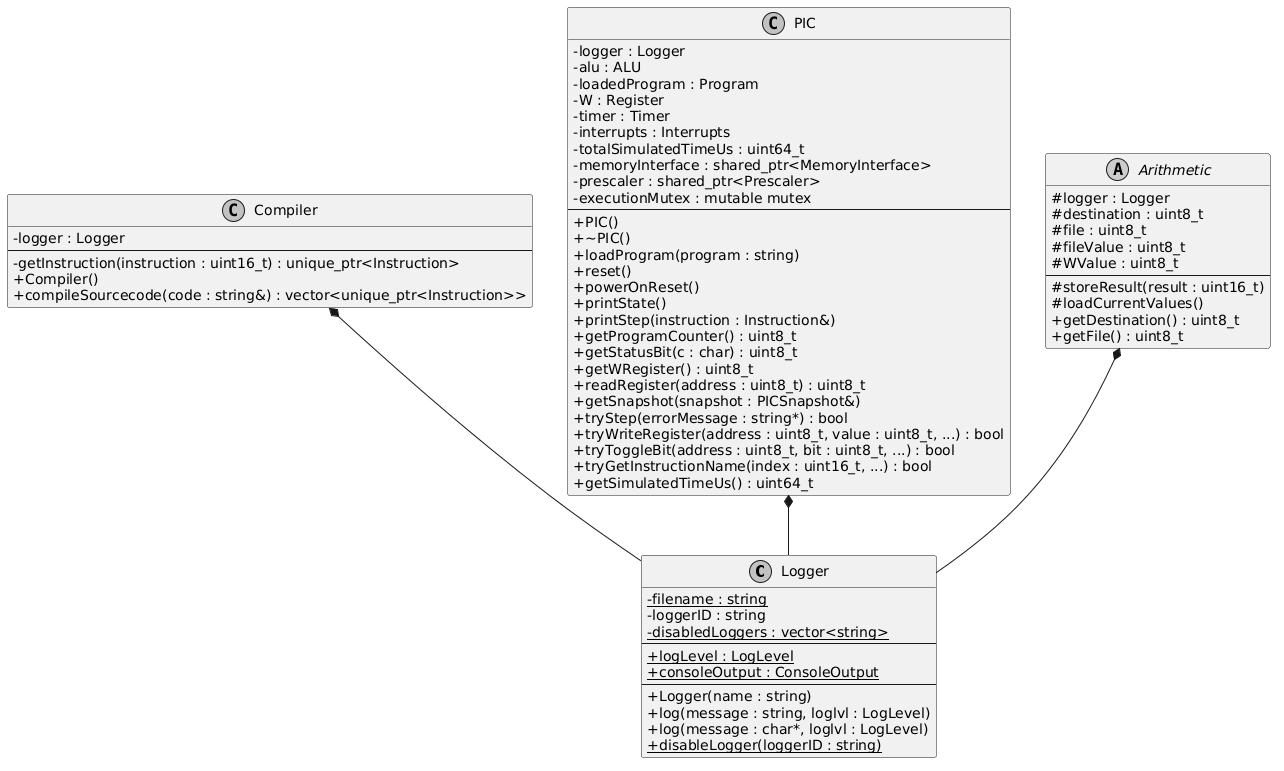
\includegraphics[width=0.9\textwidth]{UML/11.png}
\end{center}

\section{DRY}

\textbf{Beispiel: (Commit: ed2bead79cd82429ca9a1f6071dcb06d4e7ba7f0)} throwErrors Funktion in der Ram Klasse.

\textbf{Vorher (duplizierter Code):} Ohne die Funktion wurde in jeder anderen Funktion der identische Code ausgeführt, um Fehler zu erkennen.


\begin{lstlisting}[style=codeblock,language=picassocpp]
uint8_t Ram::readRegister(uint8_t address)
{
    if (isOutOfScope(address))
        throw std::runtime_error("Address out of range");

    if (!memory[readBankSelectBit()][address])
    {
        throw std::runtime_error("Nullpointer access at address 0x" +
                                 std::to_string(address));
    }

    return memory[readBankSelectBit()][address]->readByte();
}

uint8_t Ram::readRegister(uint8_t address, bool bank)
{
    if (isOutOfScope(address))
        throw std::runtime_error("Address out of range");

    if (!memory[bank][address])
    {
        throw std::runtime_error("Nullpointer access at address 0x" +
                                 std::to_string(address));
    }

    return memory[bank][address]->readByte();
}
\end{lstlisting}

\textbf{Nachher (DRY durch Funktionsauslagerung):}

\begin{lstlisting}[style=codeblock,language=picassocpp]
uint8_t Ram::readRegister(uint8_t address)
{
    throwErrors(address);
    return memory[readBankSelectBit()][address]->readByte();
}

uint8_t Ram::readRegister(uint8_t address, bool bank)
{
    throwErrors(address, bank);
    return memory[bank][address]->readByte();
}
\end{lstlisting}

\textbf{Auswirkung:} Die Fehlererkennung wird an einer lokalen Stelle durchgeführt und kann besser angepasst werden, ohne teile zu vergessen.


\chapter{Unit Tests}

\section{10 Unit Tests}

\begin{longtable}{|p{0.05\textwidth}|p{0.26\textwidth}|p{0.18\textwidth}|p{0.41\textwidth}|}
\hline
\textbf{\#} & \textbf{Test} & \textbf{Datei} & \textbf{Beschreibung} \\
\hline
1 & \code{Bit initialisiert korrekt} & \code{test_bit.cpp} & Prüft, ob ein neu erstelltes \code{Bit}-Objekt mit \code{false} initialisiert wird. \\
\hline
2 & \code{Bit kann gesetzt werden (true)} & \code{test_bit.cpp} & Setzt ein Bit auf \code{true} und verifiziert den Wert. \\
\hline
3 & \code{Bit kann gesetzt werden (false)} & \code{test_bit.cpp} & Setzt ein Bit auf \code{false} und verifiziert, dass es \code{false} bleibt. \\
\hline
4 & \code{Nibble default constructor initializes to 0} & \code{test_nibble.cpp} & Prüft, ob ein Nibble (4 Bit) standardmäßig mit 0 initialisiert wird. \\
\hline
5 & \code{Nibble setBit and getBit} & \code{test_nibble.cpp} & Setzt einzelne Bits eines Nibbles und prüft sowohl einzelne Bits als auch den Gesamtwert (z.B. \code{0b0101}). \\
\hline
6 & \code{Byte default constructor} & \code{test_byte.cpp} & Prüft, ob \code{getByte()}, \code{getLowNibble()} und \code{getHighNibble()} jeweils 0 zurückgeben. \\
\hline
7 & \code{Byte setByte and getByte} & \code{test_byte.cpp} & Setzt \code{0xAB}, prüft ob \code{getLowNibble()} = \code{0xB} und \code{getHighNibble()} = \code{0xA}. \\
\hline
8 & \code{Byte setBit and getBit} & \code{test_byte.cpp} & Setzt Bits 0, 3, 4, 7 auf true und verifiziert, dass \code{getByte()} == \code{0x99} (10011001). \\
\hline
9 & \code{Ram reset initializes memory correctly} & \code{test_ram.cpp} & Prüft initiale Registerwerte: STATUS (0x03) hat Bits 3+4 gesetzt, TRISA (0x85)=0x1F, TRISB (0x86)=0xFF. \\
\hline
10 & \code{Read and write registers} & \code{test_ram.cpp} & Schreibt \code{0xAB} an Adresse \code{0x10}, liest zurück und vergleicht; testet unabhängige Register. \\
\hline
\end{longtable}

\section{ATRIP: Automatic, Thorough und Professional}

\subsection{Automatic}

Alle Tests laufen vollautomatisch über das Catch2-Framework. Mit dem Befehl \code{./build/AllTests} im project root werden alle Tests ausgeführt, ohne manuelle Konfiguration. Das CMake-Build-System registriert die Tests automatisch via \code{catch_discover_tests()} in der \code{CTestTestfile.cmake}, sodass auch \code{ctest} verwendet werden kann. Keine manuellen Schritte, Eingaben oder Inspektionen sind nötig -- jeder Test besteht oder schlägt fehl mit klarer Fehlermeldung.

\subsection{Thorough}

Die Tests decken mehrere Abstraktionsebenen ab:

\begin{itemize}
    \item \textbf{Bit-Level:} Einzelne Bits setzen/lesen
    \item \textbf{Nibble-Level:} 4-Bit-Blöcke verwalten
    \item \textbf{Byte-Level:} High/Low-Nibbles, Einzelbit-Zugriff, Gesamtbyte
    \item \textbf{RAM-Level:} Initiale Werte, Lese-/Schreiboperationen, Bankwechsel
    \item \textbf{Integrationstests:} Vollständige Programme (\code{test_validate.cpp}) mit JSON-Testdaten prüfen W-Register, Statusflags und RAM nach jeder Instruktion
\end{itemize}

\textbf{Testabdeckung:} Die Memory-Hierarchie (Bit$\rightarrow$Nibble$\rightarrow$Byte$\rightarrow$Register$\rightarrow$Ram) ist gut abgedeckt. Verbesserungspotenzial besteht bei der Abdeckung einzelner Instruktionen (z.B. dedizierte Tests für ADDWF-Carry, SUBWF-Borrow, etc.) und beim Timer/Prescaler-Subsystem.

\subsection{Professional}

Die Tests folgen guten Praktiken:

\begin{itemize}
    \item \textbf{Aussagekräftige Namen:} \code{"Bit initialisiert korrekt"}, \code{"Byte setByte and getByte"}
    \item \textbf{SECTION-Blöcke:} Gruppieren verwandte Assertions (z.B. Nibble-Setzungen in true/false/Mischfälle)
    \item \textbf{Unabhängigkeit:} Jeder Test erstellt seine eigenen Objekte -- kein gemeinsamer State
    \item \textbf{Datengetriebene Tests:} \code{test_validate.cpp} verwendet \code{GENERATE(from_range(files))} für automatische Parametrisierung über alle JSON-Testdateien
    \item \textbf{Klare REQUIRE-Assertions:} Jede Prüfung hat einen eindeutigen erwarteten Wert
\end{itemize}

\section{Fakes und Mocks}

\textbf{Fake 1: FakeMemoryInterface}

Um Instruktionen isoliert testen zu können, ohne das vollständige RAM-System aufzubauen, kann ein \code{FakeMemoryInterface} erstellt werden, das die gleiche Schnittstelle wie \code{MemoryInterface} bietet, aber intern eine einfache \code{std::map<uint8_t, uint8_t>} verwendet.

\begin{lstlisting}[style=codeblock,language=picassocpp]
class FakeMemoryInterface : public MemoryInterface {
    std::map<uint8_t, uint8_t> fakeMemory;
public:
    uint8_t readRegister(uint8_t addr) override { return fakeMemory[addr]; }
    void writeRegister(uint8_t addr, uint8_t val) override { fakeMemory[addr] = val; }
    // Statusbits als einfache Variablen
};
\end{lstlisting}

\textbf{Begründung:} Ermöglicht das Testen einzelner Instruktionen ohne Seiteneffekte auf echten RAM. Der Fake vereinfacht die Initialisierung und erlaubt exakte Kontrolle über jeden Registerwert.

\umlplaceholder{UML: IMemoryInterface $\triangleleft$-- FakeMemoryInterface | IMemoryInterface $\triangleleft$-- MemoryInterface | Instruction $\rightarrow$ IMemoryInterface}

\textbf{Fake 2: FakeProgram}

Für Tests, die die \code{PIC::tryStep()}-Logik prüfen, kann ein \code{FakeProgram} verwendet werden, das fest vorgegebene Instruktionen zurückgibt, ohne eine .LST-Datei parsen zu müssen.

\begin{lstlisting}[style=codeblock,language=picassocpp]
class FakeProgram {
    std::vector<std::unique_ptr<Instruction>> instructions;
public:
    void addInstruction(std::unique_ptr<Instruction> instr) {
        instructions.push_back(std::move(instr));
    }
    Instruction& getInstructionAt(uint16_t idx) {
        return *instructions.at(idx);
    }
    uint16_t getProgramLength() { return instructions.size(); }
};
\end{lstlisting}

\textbf{Begründung:} Macht Tests unabhängig vom Dateisystem und vom Compiler. Die Testdaten werden direkt im Test definiert, was die Tests schneller und deterministischer macht.


\chapter{Domain Driven Design}

\section{Ubiquitous Language}

\begin{longtable}{|p{0.2\textwidth}|p{0.34\textwidth}|p{0.36\textwidth}|}
\hline
\textbf{Bezeichnung} & \textbf{Bedeutung} & \textbf{Begründung} \\
\hline
\code{Register} & 8-Bit-Speicherzelle im RAM des PIC-Mikrocontrollers & Zentraler Begriff der PIC-Hardware; wird in Datenblatt, Code und Kommunikation einheitlich verwendet. \\
\hline
\code{W} (Working Register) & Der Akkumulator-Register des PIC, über den alle arithmetischen Operationen laufen & Standardbezeichnung in der PIC-Architektur; im Code als \code{Register W} in der PIC-Klasse modelliert. \\
\hline
\code{Stack} & 8-Level-Hardware-Stack für Rücksprungadressen bei CALL/RETURN & Direkt aus der PIC-Hardware übernommen; gleichnamig im Code als Klasse \code{Stack}. \\
\hline
\code{Prescaler} & Vorteilerzähler, der die Eingangsfrequenz für Timer0 oder Watchdog herunterteilt & PIC-spezifischer Fachbegriff; im Code 1:1 als Klasse \code{Prescaler} mit \code{TMR0}/\code{WDT} Source modelliert. \\
\hline
\end{longtable}

\section{Repositories (1,5P)}

Die Applikation enthält \textbf{kein Repository} im DDD-Sinne. Begründung:

Ein Repository dient dem persistenten Speichern und Abrufen von Domain-Objekten (z.B. aus einer Datenbank). PICasso ist ein Echtzeit-Simulator, der den Zustand des Mikrocontrollers vollständig im Arbeitsspeicher hält. Es gibt keine Persistenzschicht: Programme werden bei jedem Start neu aus \code{.LST}-Dateien geladen, und der Simulationszustand wird nicht gespeichert. Die Domäne eines Hardware-Simulators erfordert keinen dauerhaften Speicher für Domain-Objekte -- der Zustand existiert nur während der Laufzeit, genau wie bei echter Hardware.

\section{Aggregates (1,5P)}

\textbf{Aggregate: \code{MemoryInterface}} als Aggregate Root über \code{Ram} und \code{Stack}.

\code{MemoryInterface} bildet eine transaktionale Grenze um den gesamten Speicherzustand: Es enthält \code{Ram} (2 Bänke $\times$ 80 Register) und \code{Stack} (8-Level). Alle Zugriffe auf den Speicher laufen über \code{MemoryInterface} -- direkter Zugriff auf \code{Ram} oder \code{Stack} von außen ist nicht vorgesehen. Dadurch stellt \code{MemoryInterface} die Konsistenz des Speicherzustands sicher (z.B. Bank-Switching, Registerspiegelung, Program Counter Synchronisation).

\begin{center}
    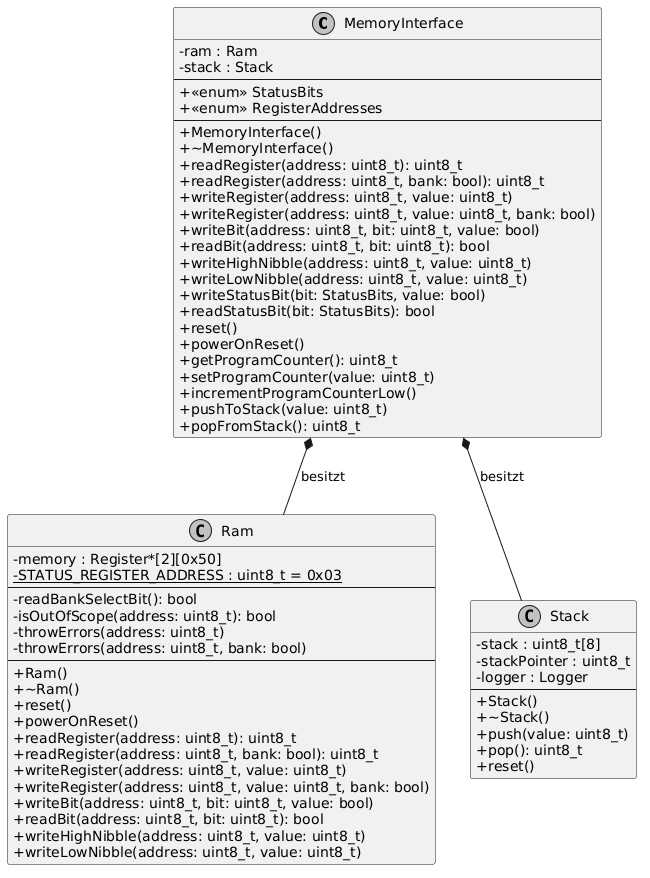
\includegraphics[width=0.9\textwidth]{UML/14.png}
\end{center}

\section{Entities (1,5P)}

\textbf{Entity: \code{PIC}}

Die \code{PIC}-Klasse repräsentiert eine konkrete Instanz eines PIC-Mikrocontrollers mit eigenem Zustand (RAM-Inhalt, W-Register-Wert, Program Counter, Simulationszeit). Zwei PIC-Instanzen mit identischem Aufbau unterscheiden sich durch ihren Zustand -- sie haben eine \textbf{Identität}, die über ihren Lebenszyklus bestehen bleibt. Der PIC durchläuft verschiedene Zustände (Power-On-Reset, laufende Simulation, Halt), behält aber seine Identität.

\begin{center}
    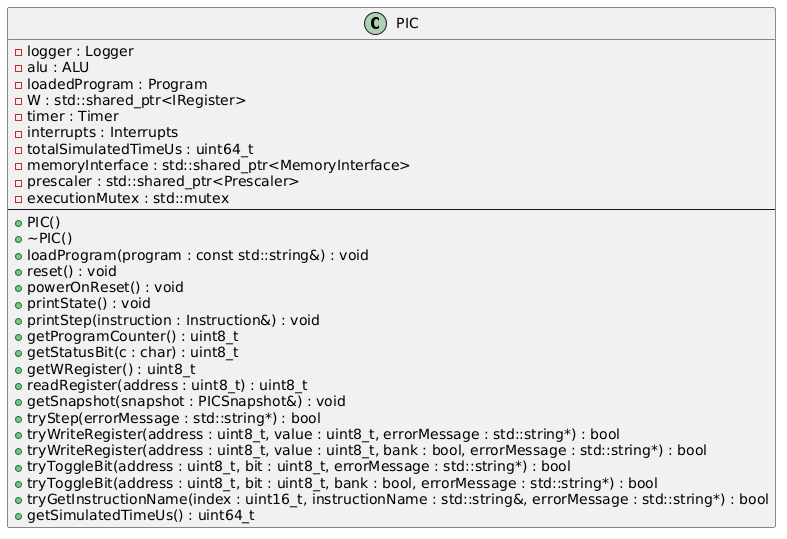
\includegraphics[width=0.9\textwidth]{UML/12.png}
\end{center}

\section{Value Objects (1,5P)}

\textbf{Value Object: \code{Bit}} (\code{header/memory/bit.hpp})

Die Klasse \code{Bit} ist ein klassisches Value Object:

\begin{itemize}
    \item \textbf{Immutability-Tendenz:} Ein Bit hat nur einen Wert (\code{true}/\code{false}), der seinen gesamten Zustand definiert.
    \item \textbf{Keine Identität:} Zwei Bits mit dem Wert \code{true} sind austauschbar -- es gibt keinen Grund, sie zu unterscheiden.
    \item \textbf{Gleichheit durch Wert:} Bits werden anhand ihres Wertes verglichen, nicht per Referenz.
\end{itemize}

Ebenso sind \code{Nibble}, \code{Byte} und \code{Register} Value Objects, da sie ausschließlich durch ihren gespeicherten Wert definiert werden.
\begin{center}
    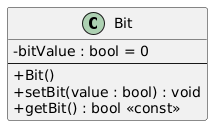
\includegraphics[width=0.5\textwidth]{UML/13.png}
\end{center}

\chapter{Refactoring}

\section{Code Smells}

\subsection{Code Smell 1: Large Class (God Object)}

Die Klasse \code{PIC} hat zu viele Verantwortlichkeiten (siehe SRP-Analyse). Sie enthält 15+ öffentliche Methoden, verwaltet 8 Felder unterschiedlicher Natur (Hardwarekomponenten, Mutex, Logger, Timing) und ist der zentrale Anlaufpunkt für fast alle Operationen.

\textbf{Lösungsweg:} Die Klasse sollte aufgeteilt werden in:

\begin{itemize}
    \item \code{PICHardware}: hält Register, RAM, Timer (Hardware-Zustand)
    \item \code{PICSimulator}: orchestriert Instruktionsausführung
    \item \code{PICDebugInterface}: bietet thread-sichere Zugriffsmethoden für die UI
\end{itemize}

\begin{lstlisting}[style=codeblock,language=picassocpp]
// Vorher: alles in PIC
class PIC {
    // Hardware-Zustand
    std::shared_ptr<ProgramCounter> pc;
    std::shared_ptr<RAM> ram;
    std::shared_ptr<Timer> timer;

    // Simulationssteuerung
    void getSnapshot(PICSnapshot& snapshot);
    bool tryWriteRegister(uint8_t addr, uint8_t val, std::string* err);
    bool tryToggleBit(uint8_t addr, uint8_t bit, std::string* err);
    bool tryStep(std::string* err);
    // ... 10+ weitere Methoden
};

// Nachher: SRP-Aufteilung
class PICHardware {
    std::shared_ptr<ProgramCounter> pc;
    std::shared_ptr<RAM> ram;
    std::shared_ptr<Timer> timer;
};

class PICSimulator {
    PICHardware& hw;
public:
    bool tryStep(std::string* err);
};

class PICDebugInterface {
    PICHardware& hw;
    PICSimulator& simulator;
    mutable std::mutex executionMutex;
public:
    void getSnapshot(PICSnapshot& snapshot);
    bool tryWriteRegister(uint8_t addr, uint8_t val, std::string* err);
    bool tryToggleBit(uint8_t addr, uint8_t bit, std::string* err);
    bool tryStep(std::string* err);
};
\end{lstlisting}

\subsection{Code Smell 2: Long Method / Switch Statement}

Die Methode \code{Compiler::getInstruction()} enthält eine lange Switch-Kaskade mit etwa 35+ Cases über mehrere Bitmask-Levels.
Dies ist ein typischer \enquote{Long Method}-Smell kombiniert mit einem \enquote{Switch Statement}-Smell.

\textbf{Lösungsweg:} Replace Conditional with Polymorphism / Registry-Pattern:

\begin{lstlisting}[style=codeblock,language=picassocpp]
// Vorher: Lange Switch-Kette in getInstruction()
switch(instruction) {
    case 0x0064: return std::make_unique<CLRWDT>(instruction);
    case 0x0009: return std::make_unique<RETFIE>(instruction);
    // ... ~35 Cases über 4 Switch-Blöcke
}

// Nachher: Factory-Registry
class InstructionRegistry {
    std::vector<std::pair<uint16_t, uint16_t, Factory>> entries;
public:
    void registerInstruction(uint16_t mask, uint16_t pattern, Factory f);
    std::unique_ptr<Instruction> create(uint16_t opcode);
};
\end{lstlisting}

\section{2 Refactorings}

\subsection{Refactoring 1: Extract Class}

\textbf{Bezeichnung:} \emph{Extract Class} – Auslagerung einer in sich geschlossenen
Teilverantwortlichkeit in eine eigene Klasse.

\textbf{Ausgangssituation:}
In \code{terminal_ui.cpp} war die gesamte Rendering-Logik als Nested-Class
\code{TerminalUI::Renderer} direkt in der Translation Unit von \code{TerminalUI}
eingebettet.  Die Nested-Class war über~300 Zeilen lang und mischte
Drawing-Verantwortung mit den übrigen Aufgaben von \code{TerminalUI}.
Das verstößt gegen das Single-Responsibility-Prinzip: Änderungen am Rendering
erforderten Anpassungen in der Hauptdatei der UI-Steuerung.

\begin{figure}[H]
  \centering
  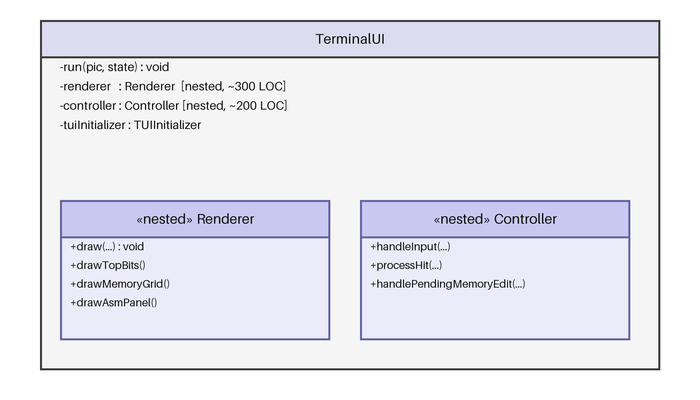
\includegraphics[width=0.55\textwidth]{UML/20.png}
  \caption{UML vor dem Refactoring: \code{Renderer} und \code{Controller} als
           Nested-Classes innerhalb von \code{TerminalUI}.}
\end{figure}

\textbf{Anwendung (Commit \texttt{2f9077e} \enquote{Extracted tui renderer class}):}
Die Nested-Class wurde als eigenständige Klasse \code{TUI_Renderer} in eigene
Dateien (\code{tui_renderer.hpp} / \code{tui_renderer.cpp}) ausgelagert.
\code{TerminalUI} hält seitdem nur noch einen \code{unique_ptr} auf das Objekt
und delegiert alle Zeichenoperationen dorthin.

\begin{lstlisting}[style=codeblock,language=picassocpp]
// Vorher: Renderer-Logik als nested class, definiert in terminal_ui.cpp
class TerminalUI {
private:
    class Renderer; // ~300 Zeilen Rendering-Code in derselben .cpp-Datei
    class Controller;
    std::unique_ptr<Renderer> renderer;
};

// Nachher: eigenstaendige Klasse in tui_renderer.hpp / tui_renderer.cpp
class TUI_Renderer {
public:
    void draw(const PICSnapshot& snapshot,
              SimulationState& state,
              const std::optional<uint8_t>& selectedRamAddress,
              const std::string& loadedPath,
              const std::vector<std::string>& fileLines,
              int manualScrollStart, bool manualScrollEnabled,
              int* renderedStart,
              std::vector<HitBox>& hitBoxes) const;
private:
    static void drawTopBits(...);
    static void drawMemoryGrid(...);
    static void drawAsmPanel(...);
    static void drawControlPanel(...);
};

class TerminalUI {
private:
    std::unique_ptr<TUI_Renderer>     renderer;    // Delegation statt Einbettung
    std::unique_ptr<TUI_Controller>   controller;
    std::unique_ptr<TUIInitializer>   initializer;
};
\end{lstlisting}

\begin{figure}[H]
  \centering
  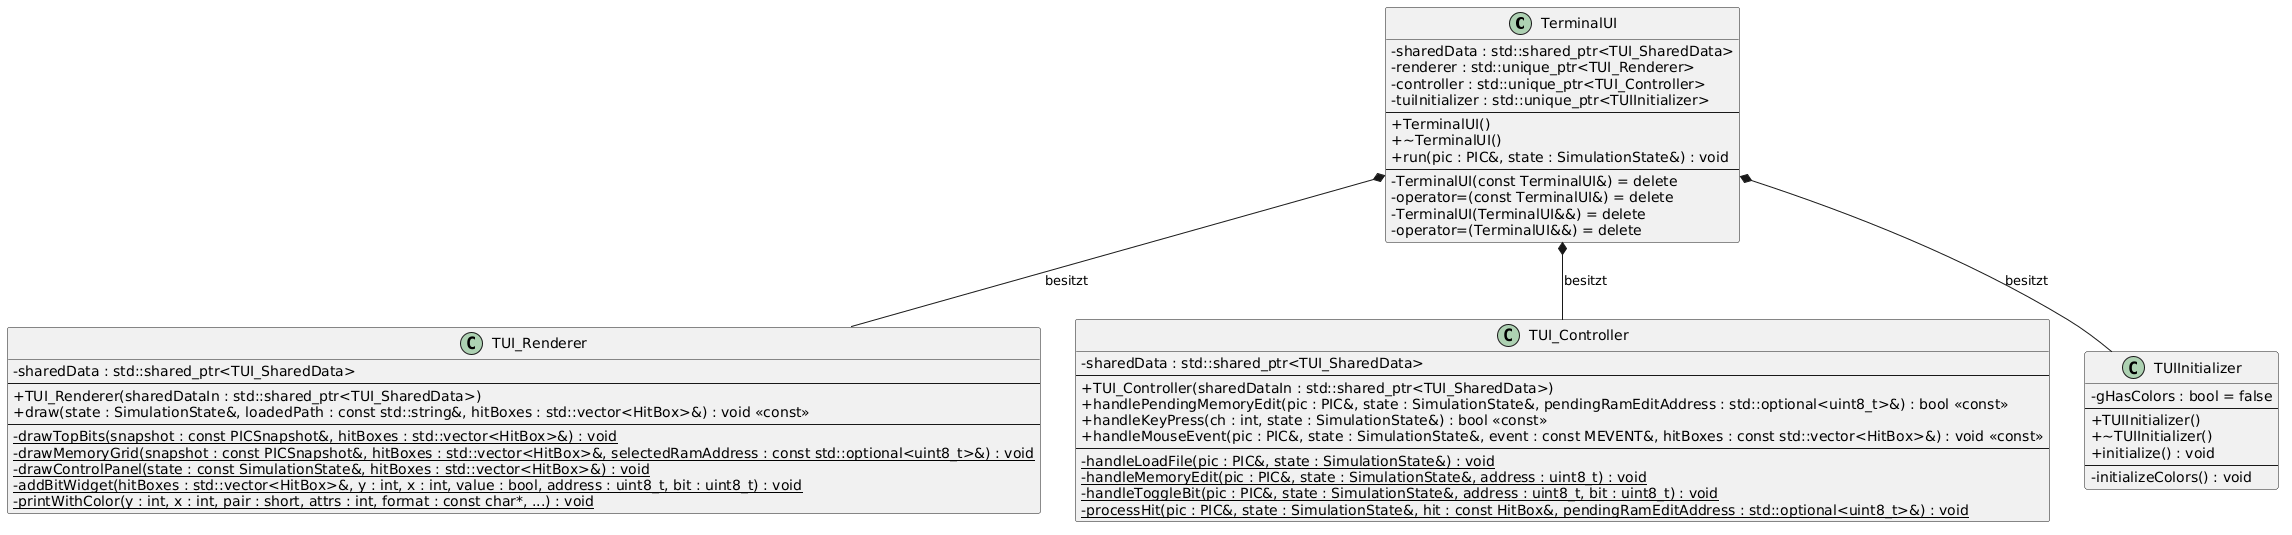
\includegraphics[height=0.3\textwidth,  angle=90]{UML/21.png}
  \caption{UML nach dem Refactoring: \code{TerminalUI} hält Kompositionsbeziehungen
           zu drei eigenständigen Klassen.}
\end{figure}

\textbf{Begründung:}
Durch die Auslagerung besitzt jede Klasse genau eine klar abgegrenzte Aufgabe.
\code{TUI_Renderer} ist unabhängig kompilierbar, separat testbar und kann
ausgetauscht werden, ohne \code{TerminalUI} anzufassen.
Die Kohäsion steigt, die Kopplung sinkt.

% -------------------------------------------------------------------

\subsection{Refactoring 2: Replace Conditional with Polymorphism}

\textbf{Bezeichnung:} \emph{Replace Conditional with Polymorphism} – Ersatz einer
expliziten Typ-Unterscheidung durch virtuellen Dispatch.

\textbf{Ausgangssituation:}
In \code{ALU::executeInstruction()} wurde nach dem Aufruf von \code{execute()}
der konkrete Typ jeder Instruktion über fünf verschachtelte
try-catch-Blöcke zur Laufzeit bestimmt.
Damit war \code{ALU} fest an alle fünf Instruktionskategorien gekoppelt: eine neue
Kategorie hätte einen weiteren Block erfordert und die Methode weiter aufgebläht.

\begin{figure}[H]
  \centering
  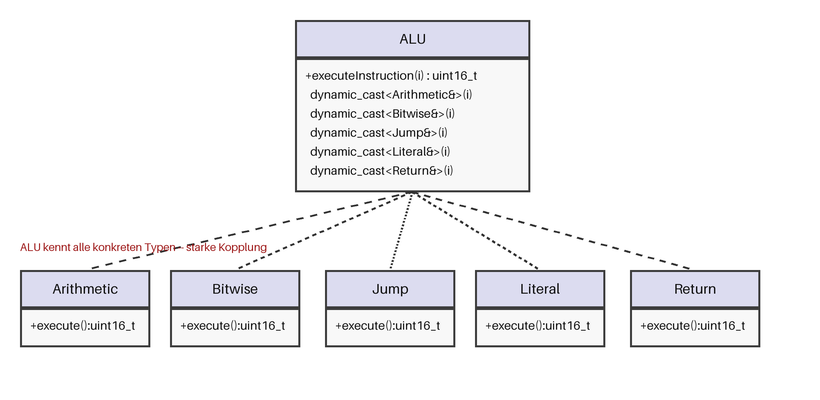
\includegraphics[width=0.82\textwidth]{UML/22.png}
  \caption{UML vor dem Refactoring: \code{ALU} kennt jeden konkreten Instruktionstyp direkt
           (starke Kopplung durch fünf \code{dynamic_cast}-Abhängigkeiten).}
\end{figure}

\textbf{Anwendung (Commit \texttt{170060b} \enquote{Basic run loop}):}
Die gesamte Typunterscheidung wurde entfernt.
Da jede konkrete Instruktionsklasse die rein virtuelle Methode \code{execute()}
der Basisklasse überschreibt, genügt der virtuelle Dispatch – \code{ALU} muss
den konkreten Typ nicht mehr kennen.

\begin{lstlisting}[style=codeblock,language=picassocpp]
// Vorher: Typabfrage per dynamic_cast nach jedem execute()-Aufruf
void ALU::executeInstruction(Instruction& instruction) {
    instruction.execute();
    std::string out = "";
    try { dynamic_cast<Arithmetic&>(instruction); out += "Arithmetic "; }
    catch (const std::bad_cast&) {}
    try { dynamic_cast<Bitwise&>(instruction);    out += "Bitwise ";    }
    catch (const std::bad_cast&) {}
    try { dynamic_cast<Jump&>(instruction);       out += "Jump ";       }
    catch (const std::bad_cast&) {}
    try { dynamic_cast<Literal&>(instruction);    out += "Literal ";    }
    catch (const std::bad_cast&) {}
    try { dynamic_cast<Return&>(instruction);     out += "Return ";     }
    catch (const std::bad_cast&) {}
    if (out == "") out = "NoFit";
    std::cout << out << std::endl;
}

// Nachher: polymorpher Dispatch genuegt vollstaendig
void ALU::executeInstruction(Instruction& instruction) {
    uint16_t executionReturn = instruction.execute();
    return executionReturn;
}
\end{lstlisting}

\begin{figure}[H]
  \centering
  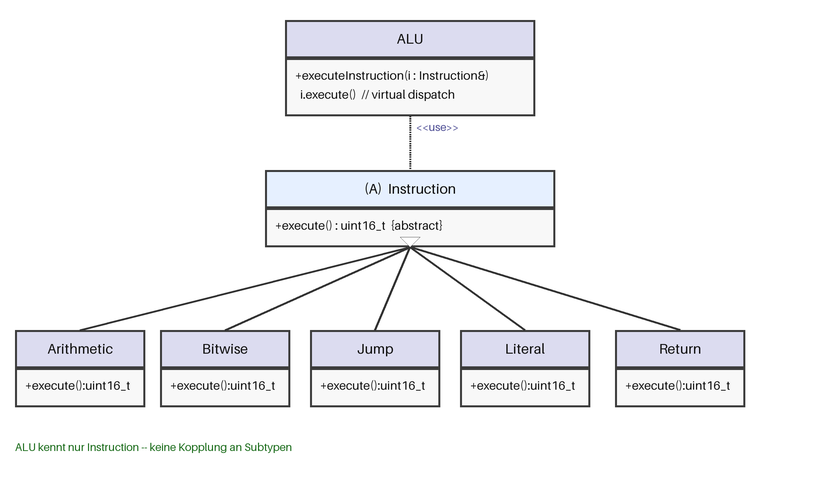
\includegraphics[width=0.72\textwidth]{UML/23.png}
  \caption{UML nach dem Refactoring: \code{ALU} kennt nur die abstrakte Schnittstelle
           \code{Instruction}; konkreter Typ ist zur Kompilierzeit irrelevant.}
\end{figure}

\textbf{Begründung:}
Mit dem virtuellen Dispatch verschwindet jede direkte Abhängigkeit der \code{ALU}
auf konkrete Instruktionsklassen.  Das Offen-Geschlossen-Prinzip wird erfüllt:
neue Instruktionskategorien können hinzugefügt werden, ohne \code{ALU} zu ändern.
Zusätzlich entfällt das ineffiziente Ausnahme-basierte Casting, das bei jedem
Schritt fünf \code{try/catch}-Blöcke durchlief.


\chapter{Entwurfsmuster}

\section{Entwurfsmuster: Kompositum Pattern}

\textbf{Einsatz:} Die Memory-Hierarchie \code{Bit -> Nibble -> Byte -> Register} implementiert ein Composite Pattern, bei dem komplexere Speichereinheiten aus einfacheren zusammengesetzt werden.

\textbf{Beschreibung:}

\begin{itemize}
    \item \code{Bit} -- speichert einen einzelnen boolschen Wert
    \item \code{Nibble} -- besteht aus einem Array von 4 \code{Bit}-Objekten
    \item \code{Byte} -- besteht aus 2 \code{Nibble}-Objekten (High + Low)
    \item \code{Register} -- besteht aus 1 \code{Byte}-Objekt
\end{itemize}

Jede Ebene bietet Zugriffsmethoden auf ihrer Abstraktionsebene (\code{getBit()}, \code{getNibble()}, \code{getByte()}) und delegiert bei Bedarf an die darunterliegende Schicht. Ein \code{Byte} kann sowohl als Ganzes (\code{setByte(0xAB)}) als auch auf Nibble- oder Bitebene manipuliert werden.

\textbf{Begründung:} Die PIC-Hardware operiert auf verschiedenen Granularitätsebenen -- Einzelbits (Status-Flags), Nibbles (BCD-Operationen), Bytes (Registerwerte). Das Composite Pattern erlaubt einheitlichen Zugriff auf allen Ebenen, ohne die Implementierungsdetails zu verletzen.


\begin{center}
    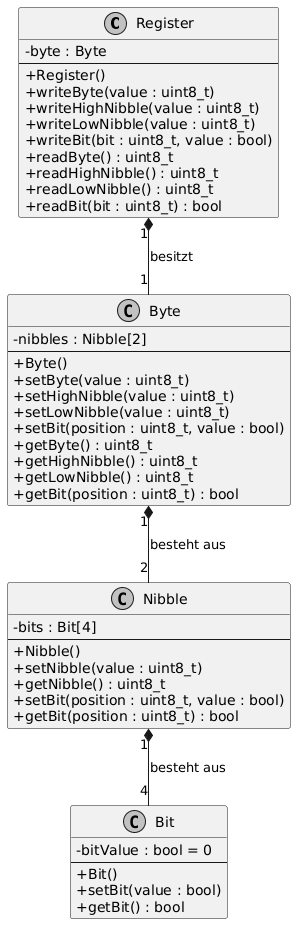
\includegraphics[width=0.5\textwidth]{UML/18.png}
\end{center}

\section{Entwurfsmuster: Strategy Pattern}

\textbf{Einsatz:} Die \code{Instruction}-Hierarchie implementiert das Strategy Pattern (bzw. Template Method Pattern) für die Ausführung verschiedener PIC-Instruktionen.

\textbf{Beschreibung:}

Die abstrakte Basisklasse \code{Instruction} definiert die Methode \code{virtual uint16_t execute() = 0}. Jede konkrete Instruktion (ADDWF, SUBWF, GOTO, CALL, BCF, BSF, etc.) implementiert ihren eigenen Algorithmus in \code{execute()}. Die \code{ALU} nutzt die Basisklasse als Schnittstelle und kann jede Instruktion polymorph ausführen, ohne den konkreten Typ zu kennen.

\begin{lstlisting}[style=codeblock,language=picassocpp]
// Strategy-Interface:
class Instruction {
    virtual uint16_t execute() = 0;
};

// Konkrete Strategien:
class ADDWF : public Arithmetic { uint16_t execute() override { /* Addition */ } };
class GOTO  : public Jump       { uint16_t execute() override { /* Sprung */ } };
class BCF   : public Bitwise    { uint16_t execute() override { /* Bit Clear */ } };

// Context (ALU):
class ALU {
    uint16_t executeInstruction(Instruction& instr) {
        return instr.execute();  // polymorphe Ausführung
    }
};
\end{lstlisting}

\textbf{Begründung:} Der PIC hat 35+ unterschiedliche Instruktionen, die alle denselben Lebenszyklus durchlaufen (Dekodierung $\rightarrow$ Ausführung $\rightarrow$ Zyklenanzahl), aber völlig unterschiedliche Algorithmen haben. Das Strategy Pattern ermöglicht das Hinzufügen neuer Instruktionen durch Erstellung neuer Klassen, ohne bestehenden Code zu ändern.


\begin{center}
    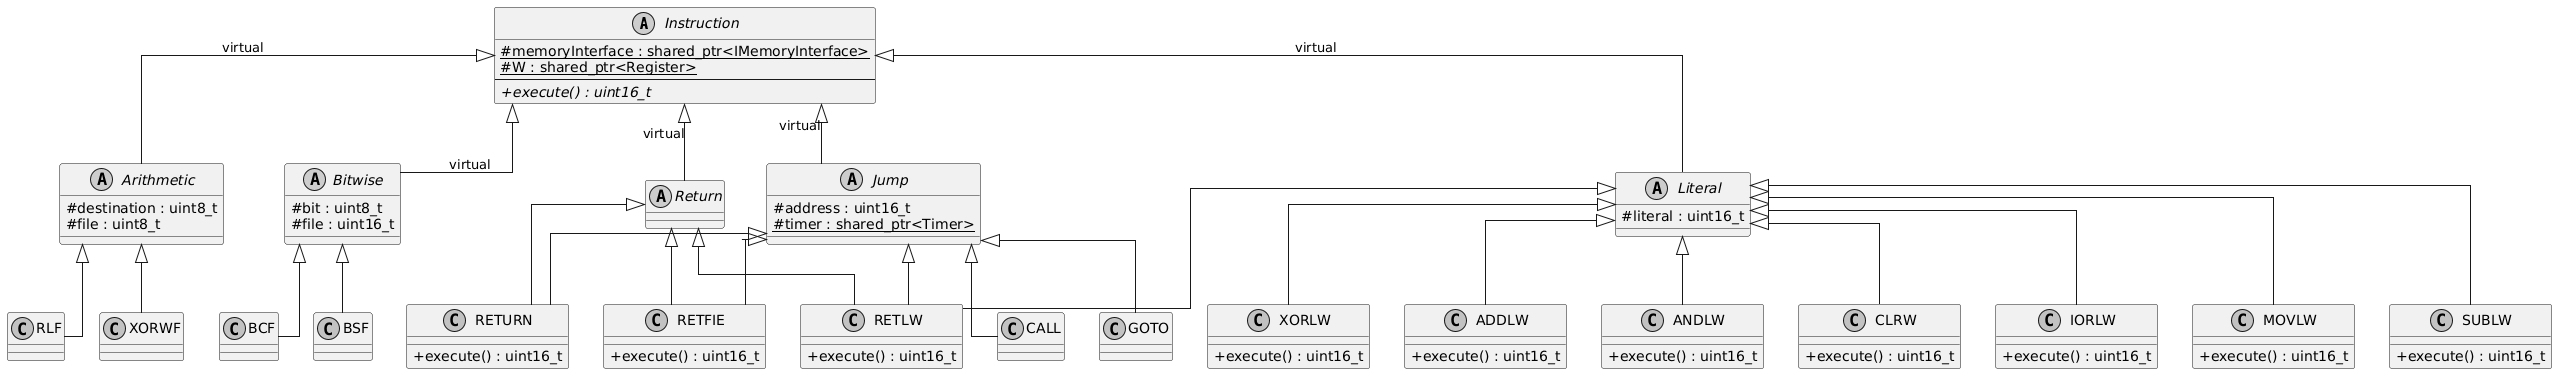
\includegraphics[height=0.25\textwidth, angle=90]{UML/19.png}
\end{center}



\end{document}
